%%% Local Variables:
%%% mode: latex
%%% TeX-master: t
%%% End:

\chapter{Implementation}

\label{ch:implementation}

\section{Architecture}

\begin{figure}[h]
\centering
  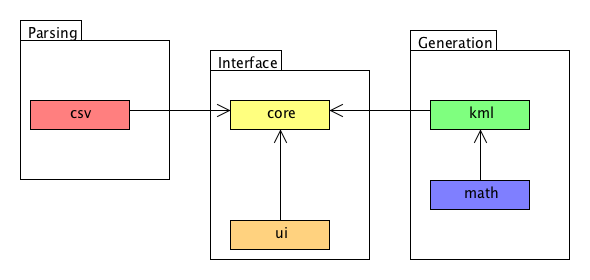
\includegraphics[scale=0.5]{gfx/fyp-arch.png}
\caption{Application architecture as a dependency graph}
\end{figure}

The application was divided into 5 main modules, or namespaces in clojure speak, with each namespace containing functions that perform a particular task. \\

As evident by the figure above, these namespaces were grouped into three broad areas; parsing, interfacing and generation. The primary motivation for having all this classification was to maintain decoupled code. The modularity also helped with keeping the code easier to extend. \\

For example, if the input format was to change, the only module effected would be the csv module. The kml, math and ui namespaces would be unaffected by this change. \\

Another broad aspect of the architecture was to keep the interfaces between the modules well defined. Therefore even though the implementation might change, things would not break.\\

\section{Parsing}

As mentioned in the requirements, the application should be able to read input from a csv file. Parsing the data by itself was pretty straightforward. Clojure comes with a very performant csv parser called clojure.data.csv which returns a sequence of vectors, representing the columns and rows in the csv data set. \\

The parser does need logic to ignore comments, as clojure.data.csv does not recognize them. Nor does it ignore whitespace. Therefore I needed to add some simple logic to filter out whitespace and comments. \\

A very important part of the dataset is the data header. This usually is the first line of the file, if whitespace and comments are ignored. The header specifies which column represents what data. \\

Therefore the csv namespace offers a function called \lstinline{read} which takes a string or a buffered reader, performs the parsing and returns a vector of hash-maps. Each hash-map represents a row, and each value in hash-map represents the value at that row for a particular column. The column names are kept as keys during this representation. \\

As the mapping between column names in the data set and what they represent in the application is not fixed,it would not be wise to hardcode that mapping in the application. The CSV file has no gurantees that the headers would remain the same for all datasets.\\

\begin{lstlisting}[caption= A sample header from the csv dataset]
"Time","Magnetic Heading (DEGS)","Pressure Altitude (feet)","GPS Latitude (degs)","GPS Longitude (degs)","AIR GROUND (0-AIR,1-GND)","Throttle Lever Position Engine 1 (DEGS)","Throttle Lever Position Engine 2 (DEGS)","Throttle Lever Position Engine 3 (DEGS)","Throttle Lever Position Engine 4 (DEGS)","Roll Angle (DEGS)","Pitch Angle (DEGS)","N1 Actual Engine 1 (\%)","N1 Actual Engine 2 (\%)","N1 Actual Engine 3 (\%)","N1 Actual Engine 4 (\%)","UTC Time  (hh:mm:ss)"
\end{lstlisting}

The application tackles this problem in two ways:
\begin{enumerate}

\item The user interface requests the user to fill in the mapping (see figure below).
\item The parser guesses which headers strings correspond to what data. The guessing logic for now is very simple. It simply checks if a field in the header contains a certain substring which would recognize that field. This is not a fool proof method by any means, but helps in reducing work for the user by auto filling the mapping section in the user interface.
\end{enumerate}

To perform the guessing, the csv namespace exposes a function called \lstinline{analyze-headers!}\\

\begin{figure}[h]
\centering
  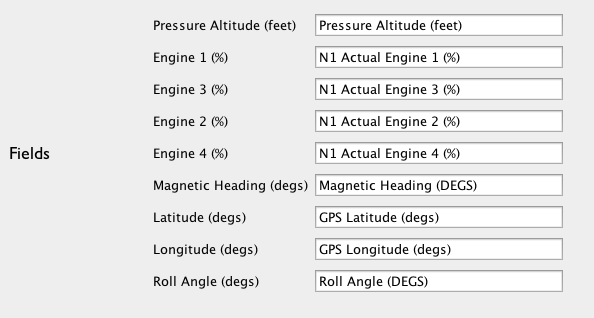
\includegraphics[scale=0.7]{gfx/ui-fields.png}
\caption{User interface allows users to specify field names in the csv file}
\end{figure}

As clojure sequences are lazy data structures, I do not need to worry about heap overflows, if the data size increases. That is the fundamental reason why clojure.data.csv returns a sequence of rows, intead of a vector, which is not lazy.\\

\section{Generation}

There are two main namespaces that classify within generation.

\subsection{math}

As should be evident by the name, this namespace largely implements the mathematical models mentioned in the previous chapter. The main functions it exposes include \lstinline{right-rect-from-edge} and \lstinline{left-rect-from-edge}. \\

\lstinline{left-rect-from-edge} takes a point, width, height, heading and roll angle to produce a rectangle that represents the left wing of an aircraft\footnote{When viewed from behind}. Similarly \lstinline{right-rect-from-edge} does pretty much the same thing for the right wing of the aircraft.\\


\subsection{kml}

This namespace contains functions that do the bulk of the KML generation. The main interface here is the \lstinline{render} function which generates the KML document and emits the result to a file. \\

The hiccup DSL is used very heavily here, along with clojure.data.xml for speedy emission. Hiccup is primarily used to build base XML components which are fed coordinates from calling functions from the  \lstinline{math} namespace. \\

 KML allows specifying styles to elements, which works like a bit like CSS. KML elements can have ids, which Style objects can refer to when they specify styles like line and fill color. Because user's would want the ability to customize colors, the \lstinline{render} function also takes a style configuration as an argument. \\

AAIB also specified in the user requirements, that users should be able to select and unselect various elemnts in the visualisation. This taken care of within this namespace through using KML's Folders to structure the document in a user friendly way. \\

\begin{figure}[h]
\centering
  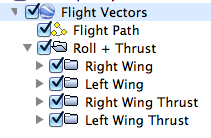
\includegraphics[scale=1]{gfx/kml-structure.png}
\caption{Users can select which components they want to view}
\end{figure}

\section{Interface}


The application needs to be able to effectively interact with users. Since the core functionality of the application is very specific, the set of possible user interactions is actually not very large. The application features the following interactions:

\begin{itemize}
\item specify input file path
\item specify output file path
\item fill field names from the CSV dataset, if they are guessed incorrectly
\item assign colors to the each of components
\item add engine configuration
\end{itemize}

Using clojure meant that Java's swing libraries were available for writing UI code. However swing by itself is incredibly verbose. Although clojure supports interoperability with Java, writing clojure code in a Java-esque fashion would defeat the purpose of using clojure in the first place. \\

Enter seesaw, a well documented clojure library and DSL that allows developers to construct swing based applications without having to deal with swing directly \citep{clj:seesaw}.\\

Seesaw's allows the creation of swing objects in a very succint fashion. Because of clojure's nature of being a lisp and running at a REPL, seesaw allows a very fast feedback loop when designing a user interface, as seesaw functions can be invoked at the REPL.\\

In addition to just creating swing object, seesaw also allows querying the tree of UI elements for specific elements. This API is inspired from CSS selectors on web browsers. One can query elements by their ids or their classes. \\

I made heavy use of seesaw when writing the code for the user interface. Which is also why I was able to keep the \lstinline{ui} namespace under 200 lines of code.\\


\begin{figure}[h]
\centering
  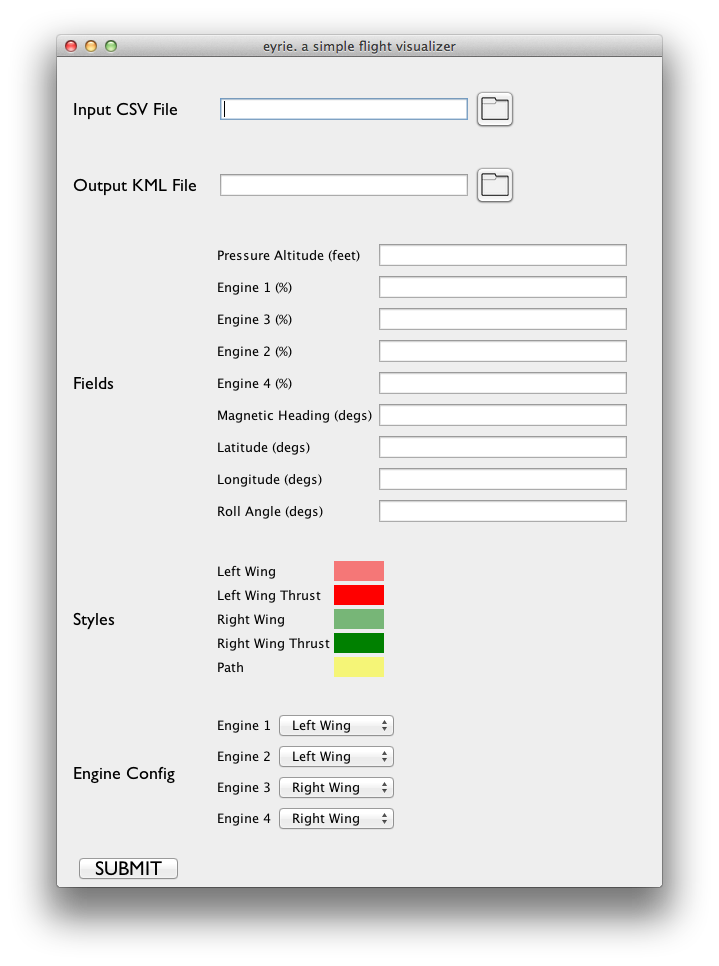
\includegraphics[scale=0.5]{gfx/ui-overview.png}
\caption{An overview of the user interface}
\end{figure}

\subsection{UI Flow}

\begin{enumerate}
\item The user launches the application
\item He/she selects an input csv file. This can be done by either writing the path to the file manually in the text box, or clicking on a button that launches a file picker. As soon as the input file is selected, the application analyses the file's headers and auto fills the fields section. \\
Under the hood, this launches a call to the \lstinline{csv/analyze-headers!} on a separate thread. This is so any processing does not freeze the interface.
\item The user enters the path he/she wants to output to.
\item The user fills up any missing fields, or corrects fields that may have been detected wrong.
\item The user chooses colors for each of the components. Clicking on colored button next to the component name launches a color picker, where the user can choose a new color for that component.
\item Lastly, the user fills up the engine configuration. This specifies which engine is on which wing.
\item The user hits submit.
\item If the file, the user selected was valid
\end{enumerate}
